%-------------------------------------------------------------------------------
%-------------------------------------------------------------------------------
\section{Matrices positives} \label{sec:LinAlg-Pos}
%-------------------------------------------------------------------------------
%-------------------------------------------------------------------------------

\remarks 
\begin{enumerate}
  \item On ne s'intéresse ici qu'à des matrices carrées : $A \in \Mcal_n$.
  \item Il existe deux acceptions du terme ``matrice positive'' :
  \begin{enumerate}[$\bullet$]
    \item matrice positive au sens du produit scalaire $A \succcurlyeq 0$
    \item matrice positive au sens de Perron-Frobénius $A \geq 0$
  \end{enumerate}
\end{enumerate}


%-------------------------------------------------------------------------------
%-------------------------------------------------------------------------------
\subsection{Matrices positives (au sens du produit scalaire : $A \succcurlyeq 0$)} 
%-------------------------------------------------------------------------------

\begin{definition}[Matrice positive] \label{def:matricePositive}
  Une matrice {\em symétrique} $A \in \Mcal_n$ est dite positive ($A \succcurlyeq 0$) ssi, 
  $$
  \forall x \in \Rbb: \quad x^\top A x \geq 0.
  $$
  Une matrice {\em symétrique} $A \in \Mcal_n$ est dite définie positive ($A \succ 0$) ssi, elle est positive et 
  $$
  x^\top A x = 0 \qquad \Leftrightarrow \qquad x = 0.
  $$
\end{definition}

\remark
On peut se demander pourquoi on restreint la définition aux matrices symétriques. La raison est que seule la {\em partie positive} d'une matrice intervient dans la définition de la positivité. \\
Pour s'en convaincre il suffit d'observer qu'on peut décomposer toute matrice $A$  en $A = S + T$ où $S$ est symétrique ($S = S^\top$) et $T$ est anti-symétrique ($T = -T^\top$) en prenant
$$
S = (A + A^\top) / 2, \qquad T = (A - A^\top) / 2
$$
(on peut d'ailleurs montrer que cette décomposition est unique). \\
La {\em forme quadratique} $x^\top A x$ s'écrit alors
\begin{align*}
  x^\top A x 
  & = x^\top S x + x^\top T x 
\end{align*}
où le second terme $x^\top T x$ est nul puisque, $x^\top T x$ étant un scalaire, il est égal à sont transposé, et donc
$$
x^\top T x = (x^\top T x)^\top = x^\top T^\top x = x^\top (- T) x = - x^\top T x.
$$

\begin{proposition}
  $A$ (symétrique) est positive (resp. définie positive) ssi toutes ses valeurs propres sont (resp. strictement) positives ou nulles. 
\end{proposition}

\proof
Puisque $A$ est symétrique, elle est diagonalisable et s'écrit $A = P^\top \Lambda P$.
\begin{description}
  \item[$\Rightarrow$:] $\lambda$ est une valeur propre de $A$ ssi, il existe $x \neq 0$ tel que
  $$
  Ax = \lambda x \qquad \Rightarrow \qquad x^\top A x = \lambda x^\top x,
  $$
  or $x^\top A x \geq 0$ et $x^\top x > 0$ donc $\lambda \geq 0$. \\
  Si $A$ est définie positive, $x^\top A x > 0$ pour tout $x$ non nul et donc $\lambda > 0$.
  \item[$\Leftarrow$:] si toutes les valeurs propres de $A$ sont (strictement) positives, on a pour tout $x \neq 0$, en posant $y = P x$:
  $$
  x^\top A x = x^\top P^\top \Lambda P x = y^\top \Lambda y = \sum_i \lambda_i y_i^2
  $$
  qui est (strictement) positif si toutes les valeurs propres sont (strictement) positives.
\end{description}
\eproof

% \begin{proposition}[Matrice positive symétrique]
%   Si $A$ est positive ($A \succcurlyeq 0$) et symétrique ($A = A^\top$), elle est est diagonalisable. De plus ses valeurs propres sont positives et ses vecteurs propres sont orthogonaux deux à deux.
% \end{proposition}
% 
% \proof
% Il suffit de combiner le dernier théorème de la section \ref{sec:MatDiag} avec la proposition précédente.
% \eproof

% \begin{proposition}[Inverse d'un matrice orthonormale] \todo{A faire en TD}
%   Si $P \in \Mcal_n$ est orthonormale, alors $P^{-1} = P^\top$.
% \end{proposition}

% \proof
% En notant $P = [v_{ij}]$, $v_j$ le $j$-ème vecteur colonne de $P$ et $B = [b_{ij}] = P^\top P$, on a
% $$
% P^\top = [v_{ji}] 
% \quad \Rightarrow \quad
% b_{ik} 
% = \sum_{k=1}^n [P^\top]_{ik} [P]_{kj} 
% = \sum_{k=1}^n v_{ki} v_{kj}
% = < v_i, v_j >
% = \left\{\begin{array}{rl} 1 & \text{si } i = j \\ 0 & \text{sinon} \end{array}\right.
% $$
% (puique les vecteurs $v_j$ sont orthonormés), donc $P^\top P = B = I$. La démonstration de $P P^\top = I$ est symétrique.
% \eproof

%-------------------------------------------------------------------------------
\subsubsection{Matrice de variance-covariance}
%-------------------------------------------------------------------------------

On revient à l'étude des matrices de variance-covariance introduite à la section \ref{sec:MatCov}.

\begin{proposition}[Matrice de variance-covariance]
  Soit $\Sigma$ la matrice de variance-covariance d'un vecteur aléatoire $X = [X_1, \dots X_n]^\top$.
  \begin{enumerate}
    \item $\Sigma$ est diagonalisable ;
    \item $\Sigma$ est positive : $\Sigma \succcurlyeq 0$ ;
    \item $\Sigma$ est définie positive sauf si une des $n$ variables est une fonction déterministe des $n-1$ autres.
  \end{enumerate}
\end{proposition}

\proof
\begin{enumerate}
\item Cela résulte du fait que $\Sigma$ est réelle et symétrique.
\item On considère un vecteur $v = [v_1 \dots v_n]^\top$ quelconque et on définit la variable aléatoire 
$$
Y = \sum_{i=1}^n v_i X_i.
$$
Sa variance est positive ou nulle et vaut
$$
0 \leq \Var Y 
= \sum_i v_i^2 \Var(X_i) + \sum_{i \neq j} v_i v_j \Cov(X_i, X_j)
= v^\top \Sigma v
$$
donc $\Sigma$ est positive.
\item Si $\Sigma$  n'est pas définie positive, alors, elle admet une valeur propre nulle et il existe un vecteur $v$ tel que $\Sigma v = 0$, donc $v^\top \Sigma v = 0$, ce qui signifie que la variable aléatoire $Y$ associée est de variance nulle, donc qu'elle est constante (et égale à $y$). On a donc
$$
\sum_i v_i X_i = y,
$$
soit, en choisissant un $v_i$ non nul: 
$$
X_i = y - \sum_{j \neq i} v_j/v_i X_j.
$$
\end{enumerate}
\eproof

% %-------------------------------------------------------------------------------
% \paragraph*{Analyse en composantes principales} \todo{A faire en TD}
% L'analyse en composantes principales consiste précisément à diagonaliser la matrice de variance (estimée) d'un vecteur aléatoire $X = [X_1 \; X_2 \; \dots \; X_n]^\top$ pour déterminer les combinaisons linéaires de plus grande variances. Pour cela, on ordonne les valeurs propres de $\Sigma = \Var(X)$ : 
% $$
% \lambda_1 \geq \lambda_2 \geq \dots \geq \lambda_n
% $$
% et on définit les composantes principales comme les vecteurs propres associés aux plus grandes valeurs propres $\lambda_1, \lambda_2, \lambda_3$.
% 
% \dessin{Exemple pour $n = 2$ : Dessin avec grand axe et petit axe de l'ellipse. Par exemple
% $$
% \Sigma = \left[\begin{array}{cc} 1 & \sqrt{7}/2 \\ \sqrt{7}/2 & \sqrt{7}/2 \end{array}\right]
% $$
% donne
% $$
% \left(\lambda_1 = \frac{9}2, \quad 
% v_1 = \frac{1}{2\sqrt{2}} \left[\begin{array}{r} 1 \\ \sqrt{7} \end{array}\right]\right), 
% \qquad
% \left(\lambda_2 = \frac{1}2, \quad 
% v_2 = \frac{1}{2\sqrt{2}} \left[\begin{array}{r} -\sqrt{7} \\ 1 \end{array}\right]\right).
% $$}
% 
% %-------------------------------------------------------------------------------
% \paragraph*{Interprétation de l'ACP.}
% La diagonalisation de $\Sigma = P D P^{-1}$ où
% $$
% D = \diag(\lambda_1, \dots \lambda_n), \qquad
% P = [v_{ij}], \qquad
% P^{-1} = [u_{ij}]
% $$
% permet de définir un vecteur aléatoire $Y = [Y_1 \; Y_2 \; \dots \; Y_n]^\top$ tel que
% $$
% Y_i = \sum_{j=1}^n u_{ij} X_j
% \qquad \Rightarrow \qquad
% Y = P^{-1} X
% \qquad \Rightarrow \qquad
% X = P Y.
% $$
% De plus les coordonnées de $Y$ sont non corrélées entre elles puisque
% $$
% \Var(Y) = \Var(P^{-1} X) = P^{-1} \Var(X) P = P^{-1} \Sigma P = P^{-1} P D P^{-1} P = D
% $$
% donc
% $$
% \Cov(Y_i, Y_j) = 0 \text{ si } i \neq j 
% \qquad \text{et} \qquad
% \Var(Y_i) = \lambda_i.
% $$
% 
% Si, de plus, $\Sigma$ est positive, mais non définie positive (elle est alors dite {\em semie-définie positive}), elle possède 0 pour valeur propre. On note $m$ l'ordre de multiplicité de $\lambda = 0$ et $r = n-m$ la somme des ordres de multiplicité des valeurs propres non-nulles ($r$ est le {\em rang} de $\Sigma$). On peut alors écrire
% $$
% X = P^{-1} Y = [v_1 \dots v_n] \left[\begin{array}{c} Y_1 \\ \vdots \\ Y_n \end{array} \right]
% $$
% sous la forme
% $$
% X = [v_1 \dots v_r] \left[\begin{array}{c} Y_1 \\ \vdots \\ Y_r \end{array} \right],
% $$
% puisque, pour $r+1 \leq j \leq n$, $\Var(Y_j) = 0 \; \Rightarrow \; Y_j = 0$.
% Les $n$ variables aléatoires $X_1, \dots X_n$ sont donc construites de façon déterministes à partir de $r < n$ variables aléatoires $Y_1 \dots Y_r$ non corrélées.
% 
% 
% %-------------------------------------------------------------------------------
% \paragraph*{Exemple.} \dessin{\url{SeedsPCA}}

%-------------------------------------------------------------------------------
%-------------------------------------------------------------------------------
\subsection{Matrices positives (au sens de Perron–Frobenius : $A \geq 0$)} 
%-------------------------------------------------------------------------------

% Théorie de Perron–Frobenius sur les matrices à coefficients positifs. Régularité, valeur propre dominante, théorème de Perron–Frobenius. Application à la dynamique des populations structurées

\begin{definition}[Matrice positive]
  Une matrice $A = [a_{ij}]$ est dite positive ('{\em non-negative}' : $A \geq 0$) si tous ses éléments sont positifs : $a_{ij} \geq 0$. \\
  Elle dite strictement positive ('{\em positive}' : $A > 0$) si tous ses éléments sont strictement positifs : $a_{ij} > 0$. 
\end{definition}

%-------------------------------------------------------------------------------
\subsubsection{Dynamique d'une population structurée}
%-------------------------------------------------------------------------------

On revient à l'exemple des modèles de dynamique d'une population structurée introduit à la section \ref{sec:MatLeslie}. On s'intéresse donc au cas où $A$ décrit la dynamique de la population structurée en $k$ catégories : 
$$
x(n) = [x_1 \dots x_k(n)]^\top, \qquad x(n+1) = A x(n)
$$
où on a
$$
x(n) = A^n x(0).
$$
Le comportement en temps long de la population $\lim_{n \to\infty} x(n)$ est contrôlé par celui de $A^n$ : $\lim_{n \to\infty} A^n$.

\begin{proposition}[Itérée d'un matrice diagonalisable]
  Si est $A \in \Mcal_k$ est diagonalisable ($A = P D P^{-1}$) et que sa plus grande valeur propre en module $\lambda_1$ est d'ordre multiplicité 1 (on parle alors de valeur propre {\em dominante} ou de Perron-Frobénius) :
  $$
  \forall i \geq 2: \qquad |\lambda_i| < |\lambda_1|.
  $$
  alors
  $$
  \lim_{n \to \infty} \lambda_1^{-n} A^n = v_1 u_1^\top \qquad (\in \Mcal_n)
  $$
  où $v_1$ est le premier vecteur colonne de $P$ et $u_1^\top$ est le premier vecteur ligne de $P^{-1}$.
\end{proposition}

\remark
La condition $\forall i \geq 2: |\lambda_i| < |\lambda_1|$ implique que $\lambda_1$ est réelle. En effet, si $\lambda_1$ est complexe, alors $\overline{\lambda}_1$ est également valeur propre et $|\overline{\lambda}_1| = |\lambda_1|$.

\proof
  Puisque $A = P D P^{-1}$, on a
  $$
  A^n = A = P D^n P^{-1}
  \qquad \text{où} \quad 
  D^n = \diag(\lambda_1^n \; \dots \; \lambda_k^n)
  $$
  et 
  $$
  \lim_{n \to \infty} \lambda_1^{-n} D^n = C = \diag(1 \; 0 \; \dots \; 0),
  $$
  donc
  $$
  \lim_{n \to \infty} \lambda_1^{-n} A^n = P C P^{-1}.
  $$
  Il reste à vérifier que
  $$
  P C P^{-1} 
  = \left[v_1 \; v_2 \; \dots v_k\right] 
  \left[\begin{array}{cccc} 1 & & & \\ & 0 & & \\ & & \ddots & \\ & & & 0 \end{array} \right] 
  \left[\begin{array}{c} u_1^\top \\ u_2^\top \\ \vdots \\ u_k^\top \end{array}\right] 
  = v_1 u_1^\top .
  $$
\eproof

%-------------------------------------------------------------------------------
\subsubsection{Perron-Frobenius}
%-------------------------------------------------------------------------------

\begin{definition}[Matrice régulière]
  Une matrice $A \in \Mcal_k$ positive ($A \geq 0$) est dite régulière s'il existe $n \in \Nbb$ tel que $A^n$ est strictement positive : $A^n > 0$.
\end{definition}

\begin{theorem}[Perron-Frobenius] \label{thm:perronFrobenius}
  Soit $A \in \Mcal_k$ un matrice positive ($A \geq 0$) et régulière:
  \begin{itemize}
    \item $A$ possède une valeur propre dominante $\lambda_1$ (réelle);
    \item Les vecteurs propres $v$ et $u$ associés à $\lambda_1$ respectivement à droite et à gauche : 
    $$
    A v = \lambda_1 v, \qquad u^\top A = \lambda_1 u^\top
    $$
    sont strictement positifs : $v > 0$, $u > 0$;
    \item de plus
    $$
    \lim_{n \to \infty} \lambda_1^{-n} A^n = v u^\top.
    $$
  \end{itemize}
\end{theorem}

\proof
Non démontré. 
\eproof

\remark
Puisque $v$ et $u$ sont strictement positifs, on peut toujours les choisir de telle manière que $\sum_i v_i = 1$.
% et $u^\top v = 1$. Il suffit, partant de $v$ et $u$ quelconque, de définir $v' = v / \sum_i v_i$, puis $u' = u / u^\top v'$.

\remark
S'agissant d'un modèle de dynamique de population $x(n) = A^n x(0)$, le théorème de Perron-Frobénieus implique que 
$$
\lim_{n \to \infty} \lambda_1^{-n} x(n) = v u^\top x(0)
$$
ce qui signifie que
\begin{itemize}
 \item asymptotiquement, la taille de chaque classe varie géométriquement à taux $\lambda_1$, qui est donc le {\em taux de croissance de la population} ; 
 \item puisque $x(0)$ est un vecteur, $u^\top x(0)$ est un scalaire, donc $x(n)$ est asymptotiquement proportionnel au vecteur $v$ (dont les coordonnées somment à 1) qui représente donc la {\em distribution stationnaire} ;
 \item les coordonnées du vecteur $u$ qui contribuent à établir la constante 
 $$
 u^\top x(0) = \sum_i u_i x_i(0)
 $$
 sont interprétées comme les {\em valeurs reproductives} des classes.
\end{itemize}

\begin{exercise*}[Dynamique d'une population structurée]
  $x(n) = (j(n), f(n), b(n)) :$ $j =$ juvéniles, $f = $ ('floaters' = flottants : non-territoriaux, puis repreoducteurs -- cf carnivores), $b = $ reproducteurs ('breeders') et
  $$
  x(n+1) = A x(n) 
  \qquad \text{avec} \qquad
  A = \left[\begin{array}{ccc} 0 & 0 & m \\ s_j & 0 & 0 \\ 0 & s_f & s_b \end{array}\right]
  $$
  où $m =$ fertilité moyenne des reproducteurs et $s_j, s_f, s_b =$ taux de survie des juvéniles, flottants et reproducteurs. \\
  Donner les conditions sur $m$, $s_j$, $s_f$ et $s_b$ pour que la population ne s'éteigne pas.
\end{exercise*}

\solution{
  On commence par remarquer que $A \geq 0$ et que $A^4 > 0$ (ne calculer que les termes non-nuls) : $A$ est donc régulière.
  \begin{description}
    \item[Polynôme caractéristique.] On cherche ensuite à savoir s'il existe une valeur propre plus grande que 1 en étudiant les racines du polynôme caractéristique
    $$
    P_A(\lambda) 
    = -\lambda \left| \begin{array}{cc} 
                        -\lambda & 0 \\ s_f & s_b - \lambda 
                      \end{array} \right|
      + m \left| \begin{array}{cc} 
                        s_j & -\lambda \\ 0 & s_f
                      \end{array} \right|
    = - \lambda^3 + s_b \lambda^2 + ms_js_f.
    $$
    La dérivée de ce polynôme est
    $$
    P'_A(\lambda) 
    = - 3 \lambda^2 + 2 s_b \lambda
    = - \lambda (3 \lambda - 2 s_b)
    $$
    qui s'annule en $\lambda = 0$ et $\lambda = 2 s_b/3 > 0$ : 
    $P_A$ est donc décroissant ($P'_A(\lambda) < 0$) avant $\lambda = 0$, puis croissant jusqu'en  $\lambda = 2 s_b/3$, puis décroissant.
    $$
    \begin{array}{c|ccccccc}
      \lambda & - \infty & & 0 & & 2 s_b/3 & & + \infty \\
      \hline
      P'_A(\lambda) & & - & 0 & + & 0 & - \\
      \hline
      P_A(\lambda) & +\infty & \qquad \searrow \qquad & ms_js_f > 0 & \qquad \nearrow \qquad & > 0 & \qquad \searrow \qquad &
    \end{array}
    $$
    % 
    \item[Racines du polynôme caractéristique.] 
    On remarque que $P_A(0) = ms_j s_f > 0$, donc il existe au plus une racine réelle, notée $\lambda_1$ qui est de plus positive. 
    $$
    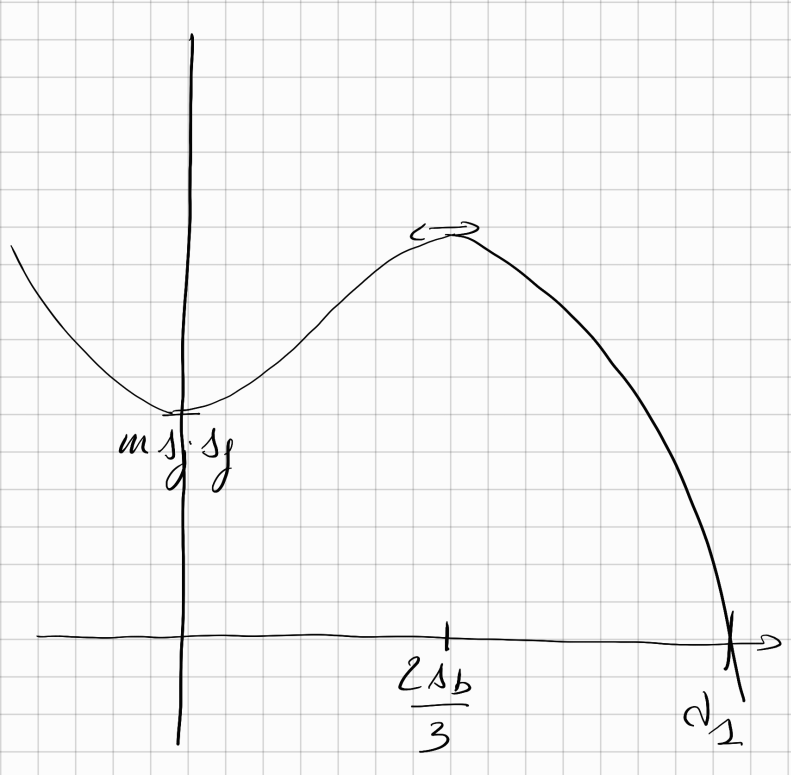
\includegraphics[width=0.4\textwidth]{DynPop3classes}
    $$
    Cette racine est plus grande que 1, si $P_A(1) >0$, c'est-à-dire si 
    $$
    -1 + s_b + ms_js_f > 0
    \qquad \Leftrightarrow \qquad
    s_b + ms_js_f > 1
    \qquad \Leftrightarrow \qquad
    \frac{ms_js_f}{1 - s_b} > 1.
    $$
    % 
    \item[Interprétation.] 
    La quantité $s_b + ms_js_f$ s'interprête comme le nombre moyen de reproducteurs engendré par un reproducteur (qui doit donc être supérieure à 1 pour assurer la surviende la population). \\
    Le rapport $m s_j s_f/(1 - s_b)$ s'interprête comme le produit du taux de transition de juvénile à reproducteur ($m s_j s_f$) par le taux de survie des reproducteurs ($1/(1 - s_b) = 1 + s_b + s_b^2 + ...$).
  \end{description}
}

% %-------------------------------------------------------------------------------
% \subsubsection{Chaîne de Markov}
% %-------------------------------------------------------------------------------
% 
% On revient maintenant aux chaînes de Markov introduites à la section \ref{sec:MatStoch} et qui seront étudiées plus en détail à la section \ref{sec:Proba-Markov}.
% 
% \begin{definition}
%   Une chaîne de Markov homogène à espace fini est une suite de variables aléatoires $\{X(n)\}_{n \geq 0}$ à valeur dans $\Xcal$ (identifié à $\{1, \dots k\}$) non indépendantes mais telles que
%   $$
%   \Pr\{X(n+1) = j \mid X(0)=x_0, X(1) = x_1) \dots X(n) = i\}
%   = \Pr\{X(n+1) = j \mid X(n) = i\}
%   = p_{ij}.
%   $$
%   La matrice $P = [p_{ij}]$ est appelée matrice de transition de la chaîne de Markov.
% \end{definition}
% 
% La matrice $P$ est une matrice stochastique car tous ses éléments sont positifs ou nuls et leur somme en ligne vaut 1 : 
% $$
% \sum_{j = 1}^k p_{ij} = 1.
% $$
% 
% \begin{proposition}
%   Soit $\mu_0$ la distribution de $X(0)$ : $\mu_{0i} = \Pr\{X(0) = i\}$ et $mu_n^{\mu_0}$ la distribution de $X(n)$ sachant la distribution initiale $\mu_0$, on a 
%   $$
%   \mu_n^{\mu_0} = \mu_0 A^n 
%   $$
% \end{proposition}
% 
% \proof
% Par récurrence, partant de $\mu_1^{\mu_0} = A \mu_0$.
% \eproof
% 
% Comme pour les modèles de dynamique des populations, le comportement de la chaîne de Markov en temps long est gouverné par par celui de $A^n$ (et par $\mu_0$).
% 
% \begin{exercise*}[1.1.14]
%   Soit $A \in \Mcal_k$ une matrice stochastique régulière. $1$ est la valeur propre dominante de $A$.
% \end{exercise*}
% 
% \solution
% \begin{enumerate}
%  \item On montre facilement que 1 est valeur propre de $A$ (car $A$ est stochastique), donc $\lambda_1 \geq 1$.
%  \item Soit $\lambda$ une valeur propre de $A$ et $v$ un vecteur propre associé, on a $A^n v = \lambda^n v$ où $A^n$ est stochastique (voir section \ref{sec:MatStoch}), donc les coordonnées de $A^n v$ sont bornées par la plus grande coordonnées de $v$, ce qui impose que $\lambda \leq 1$, donc $\lambda_1 \leq 1$.
%  \item Le fait que $A$ soit régulière assure que $\lambda_1$ est la valeur propre unique de module 1, toutes les autres ayant des modules strictement inférieurs.
% \end{enumerate}
% \esolution
% 
% \begin{proposition}
%   Si $A$ est diagonalisable, ses valeurs propres sont aussi les valeurs propres de $A^\top$ et les vecteurs propres de $A^\top$ sont les vecteurs lignes de $P^{-1}$.
% \end{proposition}
% 
% \proof
%   Il suffit de remarquer que, puique $A = P D P^{-1}$, on a 
%   $$
%   A^\top 
%   = (P D P^{-1})^\top 
%   = (P^{-1})^\top D^\top  P^\top
%   = (P^{-1})^\top D P^\top 
%   $$
%   donc $A^\top$ est aussi diagonalisable et possède les même valeurs propres (contenues dans $D$) que $A$. Pour les mêmes raisons, les vecteurs propres de $A^\top$ sont les vecteurs colonnes de $(P^{-1})^\top$, c'est à dire les vecteurs lignes de $P^{-1}$.
% \eproof
% 
% \remark
% Si $A$ est diagonalisable et que $u$ est un vecteur propre de $A^\top$, il existe $\lambda$ tel que
% $$
% A^\top u  = \lambda u 
% \qquad \Leftrightarrow \qquad
% (A^\top u)  = \lambda u^\top 
% \qquad \Leftrightarrow \qquad
% u^\top A  = \lambda u^\top 
% $$
% $u^\top$ est appelé vecteur propre {\em à gauche} de $A$ (les vecteurs propres précédemment définis étant donc des vecteurs propres {\em à droite}). Cette remarque est notamment utile pour étudier les matrice stochastiques.
% 
% Le théorème de Perron-Frobénius donne des conditions garantissant que la distribution $\mu_n$ converge vers le vecteur propre (à gauche) associé à la valeur propre 1, quelque soit la distribution initiale $\mu_0$. Ces propriétés seront étudiées en détail à la section \ref{sec:Proba-Markov}.
% 
% %-------------------------------------------------------------------------------
% \paragraph*{Exemple.}
% Succession d'espèces d'arbres (R. Arditi)
% \dessin{\url{TreeSpeciesMC}}


